\chapter{Introduction and Related Work}
\section{Describing the Flow State}
This chapter gives a brief introduction to the topic of flow, as well as related fields of work. The following chapters will answer the questions asked for this exam.

The front-runner of \textit{flow} is Mihaly Csikszentmihalyi, an Hungarian professor of psychology, whose work includes studies of happiness and creativity. He describes flow as an optimal experience, where one is in a state of control and balance: \textit{"When the information that keeps coming into awareness is congruent with goals, psychic energy flows effortlessly."} \citep{flow} He explains optimal experiences as \textit{"[s]ituations in which attention can be freely invested to achieve a person's goals, because there is no disorder to straighten out, no threat for the self to defend against."} \citep{flow} Being in flow is explained as being \textit{"completely  involved, focused, concentrating."} It's a \textit{"sense of ecstasy, of being outside everyday reality"} with \textit{"no worries about self."} \citep{ann_flow}

Flow is very much connected to challenge and skills. It can be compared to the challenge of climbing a mountain: each time a rock climber overcomes a great challenge, he is left as a more capable and skilful person \citep{flow}. While climbing the mountain, he is in a state of flow --- there is a perfect balance of what he is capable of and what is demanded of him. In other words, the difficulty of climbing the mountain fits the climber, so that it is neither too easy nor too hard. Figure \ref{fig:flowModel} shows the \textit{flow model}, which is often used when designing videogames. One should be challenged enough to not become bored. Likewise, the challenge cannot be too great compared to one's skill sets, since this will result in anxiety. In practice, one would fluctuate between these two states, but only touching them tangentially.

\begin{figure}[htbp]
\centering
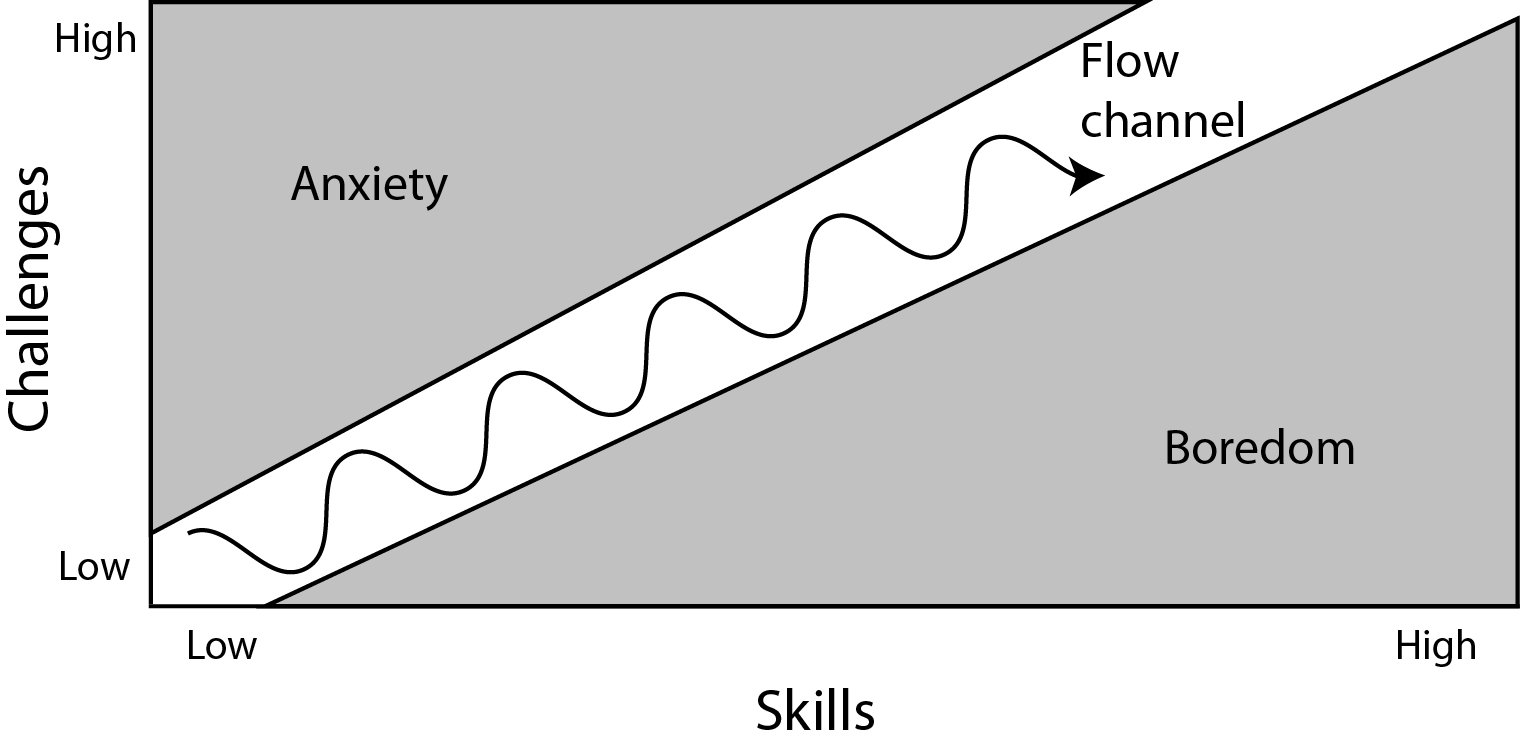
\includegraphics[width=0.70\textwidth]{Pictures/flow_model}
\caption{The flow state can be described as a balance between challenge and skills \citep{artOfGameDesign}.}
\label{fig:flowModel}
\end{figure}

\cite{flow} has found that people report extreme joy (sometimes described as "a feeling of ecstasy") in many different types of contexts. What has been found to be a common element of the activities is that they are goal-directed and bounded by rules. They are challenging activities that can not be done without the appropriate skills \citep{flow}. Additionally, they are situations with clear and immediate feedback, say, a tennis match or a game of chess. With each action, it is clear whether or not one gets closer to accomplish one's goal(s). Furthermore, the experience of enjoying the flow state often occurs in activities outside ordinary life, e.g., games and sports. Flow has been described as \textit{"[l]acking the sense of worry about losing control that is typical in many situations of normal life."} \citep{flow}. It's a sensation where one often loses self-consciousness and the sense of time and place.

A key element in experiencing flow is that the activity has an end in itself. This is described as an \textit{autotelic experience}, which means that doing something is an reward in itself. In other words, an activity should be intrinsically rewarding, where one doesn't expect external rewards, such as money or recognition by peers. Many things in life yield extrinsic rewards, i.e., we perform activities because we \textit{have} to, not because we \textit{want} to (e.g., having a boring day-job in order to earn money to live). \textit{"[I]ntrinsic motivations are not necessarily externally rewarded or supported, but nonetheless they can sustain passions, creativity, and sustained efforts."} \citep{sdt_website}

\section{Characteristics of Flow State} \label{char}
\cite{flowTwo} describe two main conditions for entering the flow state: \textit{perceived challenges that stretch, but don't overmatch, existing skills} and \textit{clear goals coupled with immediate feedback about the progress being made}. Furthermore, flow is a subjective state that is said to have the following characteristics: \citep{flowTwo}

\begin{enumerate}
\item Intense and focused concentration on the present moment
\item Merging of action and awareness
\item Loss of reflective self-consciousness (i.e., loss of awareness of oneself as a social actor)
\item A sense that one can control one's actions; that is, a sense that one can in principle deal with the situation because one knows how to respond to whatever happens next
\item Distortion of temporal experience (typically, a sense that time has passed faster than normal)
\item Experience of the activity as intrinsically rewarding, such that often the end goal is just an excuse for the process
\end{enumerate}

\section{Methods to Measure Flow}
When a person is in flow, he operates at full capacity. This state has been reported across cultures, genders and ages \citep{flowTwo}. Before the 2000's, subjective experiences (such as flow) were viewed as falling outside the sphere of scientific research. After the flow model was introduced, several self-report tools have been developed to measure flow. These include semi-structured interviews, providing a holistic account of the flow experience; and questionnaires, asking participants whether they have had any flow experience and during what contexts (e.g., "I get involved" and "I get direct clues as to how well I am doing"). Multiple scale systems have since then been developed, such as the \textit{Dispositional Flow Scale}, \textit{Flow State Scale} and \textit{Experience Sampling Method} \citep{flowTwo}. Whereas the first two consist of rating scale where participants have to retrospectively reconstruct and respond on past experiences, ESM allows for getting direct feedback by letting participants carry paging devices on them. At randomly-chosen intervals they are asked to rate their current activity, giving a clearer picture of their flow state \citep{flowTwo}.

The problem with ESM is that it risks interrupting the flow experience. That is why triangulation is needed. Several researchers are looking into ways of how to identify the flow state by looking at behavioural and/or physiological markers. Research suggests that enjoyment and involvement can be associated with significantly lower salivary cortisol levels, implying lower stress levels and low blood pressure \citep{flowTwo}.

\cite{flowTwo} find many areas promising for future research in regards to flow. E.g., neuropsychology; the nature of the attentional processes that foster flow; technology and the use of multi-tasking; autotelic personalities; addiction; and the use of flow in social environments. Furthermore, according to \cite{sdt_website}, topics such as human needs, intrinsic motivation, psychological well-being, etc., can be applied to a range of fields, including education; healthcare; relationships; psychotherapy; psychopathology; organizations; sports and exercise; goals; health and well-being; and the environment. The Self-Determination Theory is a broad framework that studies human motivation and personality. It includes meta-theories for framing motivational studies, as well as formal theories on intrinsic and extrinsic motivation, in relation to cognitive and social development. It also focuses on social and cultural factors \citep{sdt_website}.